\documentclass{report}
\usepackage[T1]{fontenc} % Fontes T1
\usepackage[utf8]{inputenc} % Input UTF8
\usepackage[backend=biber, style=ieee]{biblatex} % para usar bibliografia
\usepackage{csquotes}
\usepackage[portuguese]{babel} %Usar língua portuguesa
\usepackage{blindtext} % Gerar texto automaticamente
\usepackage[printonlyused]{acronym}
\usepackage{hyperref} % para autoreferencia
\usepackage{graphicx}
\usepackage{float}
\usepackage{subcaption}
\usepackage{makeidx}
%\setlength{\topmargin}{-20mm}
%%\usepackage[showframe]{geometry}

\addbibresource{biblatex-examples.bib}

\begin{document}
%%
% Definições
%
\def\titulo{História dos Computadores}
\def\data{23/11/2018}
\def\autores{Luis Couto  Pedro Rocha}
\def\autorescontactos{(89078) luiscouto10@ua.pt  (95057) pedromrocha@ua.pt}
\def\versao{1}
\def\departamento{\acs{deti}}
\def\empresa{Universidade de Aveiro}
\def\logotipo{ua.pdf}
\def\projeto{labi2018-ap1-g9}
%
%%%%%% CAPA %%%%%%
%
\begin{titlepage}

\begin{center}
%
\vspace*{50mm}
%
{\Huge \titulo}\\ 
%
\vspace{10mm}
%
{\Large \empresa}\\
%
\vspace{10mm}
%
{\LARGE \autores}\\ 
%
\vspace{30mm}
%
\begin{figure}[h]
\center
\includegraphics{\logotipo}
\end{figure}
%
\vspace{30mm}
\end{center}
%
\begin{flushright}
\versao
\end{flushright}
\end{titlepage}


%%  Página de Título %%
\title{%
{\Huge\textbf{\titulo}}\\
{\Large \departamento\\ \empresa}
}
%
\author{%
    \autores \\
    \autorescontactos \\
    \projeto
}
%
\date{\data}
%
\maketitle

\pagenumbering{roman}
 
\begin{abstract}
\begin{large}
Um computador é uma máquina poderosa, capaz de armazenar, recuperar e manipular informação e dados milhares de milhões de vezes mais rápido que um humano.
\paragraph{}
Neste trabalho iremos falar um pouco sobre como o computador moderno chegou a ser como é e a ter as capacidades que tem. Cada capitulo irá incidir numa época ou espaço de tempo em que foram feitos avanços significativos quer na tecnologia de \textit{hardware} quer na tecnologia de \textit{software}.
Falaremos no \textit{background} dos computadores, as máquinas de computação, e nas 5 gerações que se seguiram. Antes da primeira geração existiam apenas mecanismos de computação. A primeira geração foi marcada pelo uso de válvulas termiônicas como circuitos. A segunda geração foi marcada pela invenção e uso de transistores, a terceira pelo uso de circuitos integrados, novas linguagens de programação e pela Lei de Moore. A quarta por microprocessadores e pela \textit{internet} e a quinta por inteligencia artificial.
\paragraph{}
No final deste trabalho, será possivel concluir que os computadores modernos não foram uma invenção singular, mas sim uma obra colectiva que evolui ao longo dos anos, fruto do esforço de muitos fisicos, matemáticos e engenheiros que se dedicaram a melhorar o que já existia.
\end{large}
\end{abstract} 
 
\tableofcontents

\listoffigures

\chapter*{Acrónimos}
\begin{acronym}
\acro{deti}[DETI]{- Departamento de Electrónica, Telecomunicações e Informática}
\acro{li}[LI]{- Laboratórios de Informática}
\acro{miect}[MIECT]{- Mestrado Integrado em Engenharia de Computadores e Telemática}
\acro{ula}[ULA]{- Unidade Lógica e Aritmética}
\acro{eniac}[ENIAC]{- Electronic Numerical Integrator and Calculator}
\acro{eua}[EUA]{- Estados Unidos da América}
\acro{ram}[RAM]{- Random-Access Memory}
\acro{dram}[DRAM]{- Dynamic Random-Access Memory}
\acro{ssi}[SSI]{- Small Scale Integration}
\acro{msi}[MSI]{- Medium Scale Integration}
\acro{lsi}[LSI]{- Large Scale Integration}
\acro{vlsi}[VLSI]{- Very Large Scale Integration}
\acro{ibm}[IBM]{- International Business Machines}
\acro{so}[SO]{- Sistema Operativo}
\acro{cern}[CERN]{-  European Organization for Nuclear Research}
\acro{hp}[HP]{-  Hewlett-Packard}
\acro{gui}[GUI]{-  Graphical User Interface}
\acro{gpu}[GPU]{-  Graphics Processing Unit}
\end{acronym}

%%%%%%%%%%%%%%%%%%%%%%%%%%%%%%%% CAPITULO 1 - INTRODUÇÃO
\chapter{Introdução}
\label{chap.introducao}
\large
\section{Motivação}
\paragraph{}
No âmbito da avaliação da cadeira de \acs{li}, foi proposto efetuar um trabalho de aprofundamento, a realizar em \textit{LaTeX}, sobre um tema à escolha. 
\paragraph{}
Tendo em conta o conteúdo desta cadeira, e atendendo ao facto de o plano curricular do curso \acs{miect} ser inteiramente direcionado á formação na área das tecnologias de computação, informação e telecomunicações, achámos que seria interessante e, até de alguma importância, fazer um trabalho que se focasse na História dos Computadores, na sua evolução desde os mecanismos de computação até aos computadores que todos conhecemos e temos na actualidade.
Temos como objetivo dar a conhecer um pouco da história, das pessoas, das instituições e das invenções que tornaram possível a evolução do computador até aos niveis actuais.
\section{Estrutura do trabalho}
\paragraph{}
Quanto à estrutura, este documento está divido em 9 capítulos. Posteriormente a esta introdução, no \autoref{chap.metodologia} é apresentada a metodologia que foi seguida, e no \autoref{chap.mecanismos} são apresentados os mecanismos de computação. No \autoref{chap.PG} é discutida a primeira geração, no \autoref{chap.SG} a segunda geração e no \autoref{chap.TG} a terceira geração. No \autoref{chap.QG} é exposta a quarta geração, no \autoref{chap:IA} a quinta geração e finalmente no \autoref{chap:conclusao} a conclusão.



%%%%%%%%%%%%%%%%%%%%%%%%%%%%%%%% CAPITULO 2 - METODOLOGIA

\chapter{Metodologia}
\label{chap.metodologia}
\section{Trabalho de Pesquisa}
\paragraph{}
Sendo este um trabalho de aprofundamento sobre um dado tema, neste caso a História dos Computadores, e considerando que tem uma dimensão considerável (4000+ palavras), foi estabelecido, de modo a facilitar o igual envolvimento e distribuição de trabalho, que a pesquisa seria divida em várias tarefas e cada elemento do grupo ficaria encarregue de um certo número de tarefas. Cada elemento fez a sua própria pesquisa e completou as suas tarefas de maneira individual, sendo que existiu, no entanto, uma comunicação contínua dentro do grupo de modo a manter coerência do trabalho.
\section{Organização da informação individual}
\paragraph{}
Sendo que o nosso trabalho incide maioritáriamente na evolução dos computadores distribuida por gerações, a exposição da informação recolhida é feita de uma maneira em que existe o desenvolvimento do tema por ordem cronológica, havendo também a menção de pessoas e instituições, assim como criações, concepções e linguagens de programação que foram importantes na época e fulcrais para o desenvolvimento do computador. Apresentamos também os pontos cruciais de cada geração.
\section{Produção do trabalho final}
\paragraph{}
O resultado da pesquisa que foi realizada individualmente, de modo a concretizar o trabalho final, foi implementado em conjunto, assim como pequenas mudanças na estruturação que eventualmente se mostraram necessárias.

%%%%%%%%%%%%%%%%%%%%%%%%%%%%%%%%%%%%%%% CAPITULO 3 - MECANISMOS DE COMPUTAÇÃO 

\chapter{Mecanismos de computação}
\label{chap.mecanismos}
\section{Pavimentar o caminho}
\paragraph{}
Computadores na forma de \textit{desktops}, portáteis ou tablets são hoje aparelhos que se encontram presentes em todo o lado, quer em casa, quer no local de trabalho, e tornaram-se tão indespensáveis que é dificil pensar numa altura em que não existiam.
De facto, muito longe dos dispositivos que são hoje comumente reconhecidos como um computador, já existiam, antes do século \textit{XX}, várias máquinas de computação, usadas para realizar operações aritméticas como a adição, a subtração, a multiplicação e a divisão e até mesmo calcular funções polinomiais. 
Estas máquinas foram pioneiras na sua epóca e demonstraram ser importantes na história da computação.


\subsection{Abacus}
\paragraph{}
Reconhecido como o primeiro dispositivo com capacidade de realizar cálculos aritméticos, o primeiro \textbf{\textit{Abacus}}~\ref{abacus} \cite{Abacus}, foi datado entre um período de 2700-2300 a.C na região da Mesopotâmia e era capaz de realizar operações de adição e subtração simples. Ao longo dos séculos várias civilizações (Grega, Chinesa, Romana, Nativo Americana, etc.) usaram este dispositivo, fazendo melhorias e incrementando funcionalidades, tornando o \textbf{\textit{Abacus}} cada vez mais complexo. No entanto este dispositivo nunca foi capaz de realizar cálculos muito avançados pelo que foi sendo cada vez menos utilizado.

\begin{figure}[H]
\centering
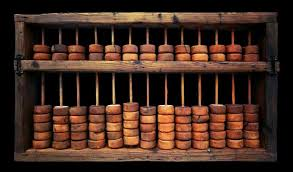
\includegraphics[width=9cm,scale=1]{Abacus.jpeg}
\caption{Abacus}
\label{abacus}
\end{figure}

\paragraph{}

\subsection{La Pascaline e Stepped Reckoner} 
\paragraph{}
Séculos á frente, entre o período de 1642-1645, nasceu ás mãos do famoso francês, matemático-filósofo, \textbf{\textit{Blaise Pascal}}, a primeira cálculadora a ser produzida e distribuida. Denominada de \textbf{\textit{La Pascaline}}~\ref{pascaline} \cite{LaPascaline}, era capaz de fazer a adição e subtração de dois números diretamente. 
\paragraph{}
Uma das maiores inovações de Pascal nesta calculadora foi o seu mecanismo de transporte, que permitiu que cada digito fosse autónomo em relação ao estado dos outros, possibilitando o transporte rápido entre digitos, independentemente da memória da calculadora.
Esta foi uma invenção muito importante na época, pois serviu de inspiração direta ou modelo base para outras calculadoras que viriam mais tarde a ser inventadas.
\paragraph{}
Alguns anos mais tarde, no período de 1672-1694 foi concebida outra calculadora mais complexa. O alemão \textbf{\textit{Gottfried Leibniz}}, também matemático-filósofo, construiu a \textbf{\textit{Step Reckoner}}~\ref{reckoner} \cite{StepReckoner}, uma calculadora expandida a partir da invenção de Pascal, que já era capaz de fazer as 4 operações aritméticas (adição, subtração, multiplicação e divisão). Para realizar efetuar multiplicações  a máquina funcionava através de adições sucessivas, sendo que para efetuar divisões funcionava através de subtrações sucessivas. \newline
Um facto interessante a ter em conta é que, apesar de não o usar na sua calculadora,  \textbf{\textit{Leibniz}} acreditava que o sistema binário era o sistema mais apropriado para máquinas de computação, o que revela o seu pensamento avançado em relação á epoca.

\begin{figure}[!htb]
   \begin{minipage}{0.5\textwidth}
     \centering
     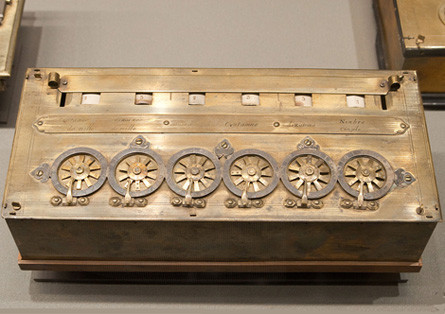
\includegraphics[width=.6\linewidth]{Pascaline.jpg}
     \caption{La Pascaline}
     \label{pascaline}
   \end{minipage}\hfill
   \begin{minipage}{0.5\textwidth}
     \centering
     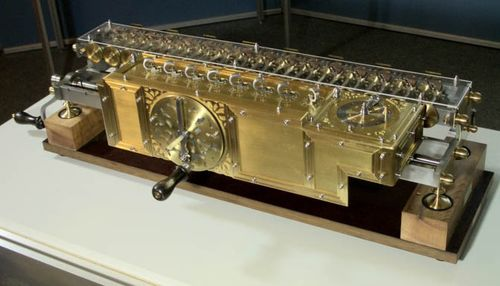
\includegraphics[width=.73\linewidth]{SteppedReckoner.jpeg}
     \caption{Stepped Reckoner}
     \label{reckoner}
   \end{minipage}
\end{figure}


\subsection{Primeiro Computador Mecânico Programával} 
\paragraph{}
Foi só no século \textit{XIX}, mais concretamente no ano de 1822, que a evolução do computador iria começar a dar os seus maiores passos. \textbf{\textit{Charles Cabbage}}, considerado por muito como o “Pai do Computador”, desenvolveu a primeira máquina de computação automática, a \textbf{\textit{Máquina Diferencial}}~\ref{diferencial} \cite{Cabbage}. \newline
Esta máquina, feita para calcular e tabelar funções polinomiais, era capaz de obter tabelas de valores aproximados de um grande número de funções matemáticas (logaritmos, funções trigonométricas, etc.), dado que estas podiam ser aproximadas por polinómios, e adicionalmente podia produzir cópias físicas desses resultados. \newline
Apesar de ter feito os planos desta máquina, \textbf{\textit{Cabbage}} nunca completou totalmente a sua construção, algo feito em Londres cerca de 150 anos depois, e que provou que a sua invenção teria funcionado.
\paragraph{}
Porém este não foi o seu maior feito. Em 1834 concebeu a \textbf{\textit{Máquina Analítica}}~\ref{analitica} \cite{Cabbage}, um engenho que funcionava através de cartões perfurados e que apresentava caracteristicas essenciais presentes em computadores modernos tais como a \acs{ula}, a memória integrada e o controlo de fluxo, sendo capaz de fazer iterações, processação paralela, conditional branching, etc.
Apesar de nunca ter sido construida enquanto \textbf{\textit{Cabbage}} era vivo, esta máquina ficou conhecida como o primeiro computador mecânico programável.

\begin{figure}
\centering
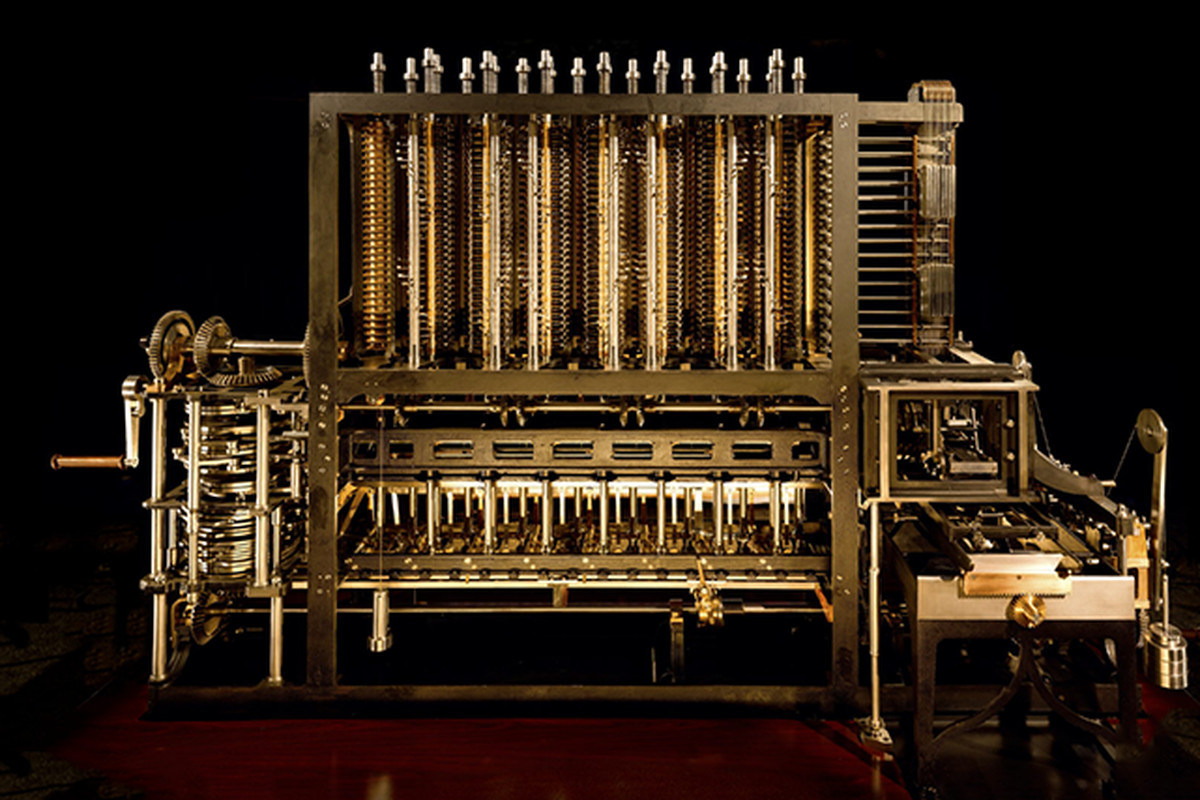
\includegraphics[width=0.7\linewidth]{Diferencial.png}
\caption{Máquina Diferencial}
\label{diferencial}
\end{figure}

\begin{figure}
\centering
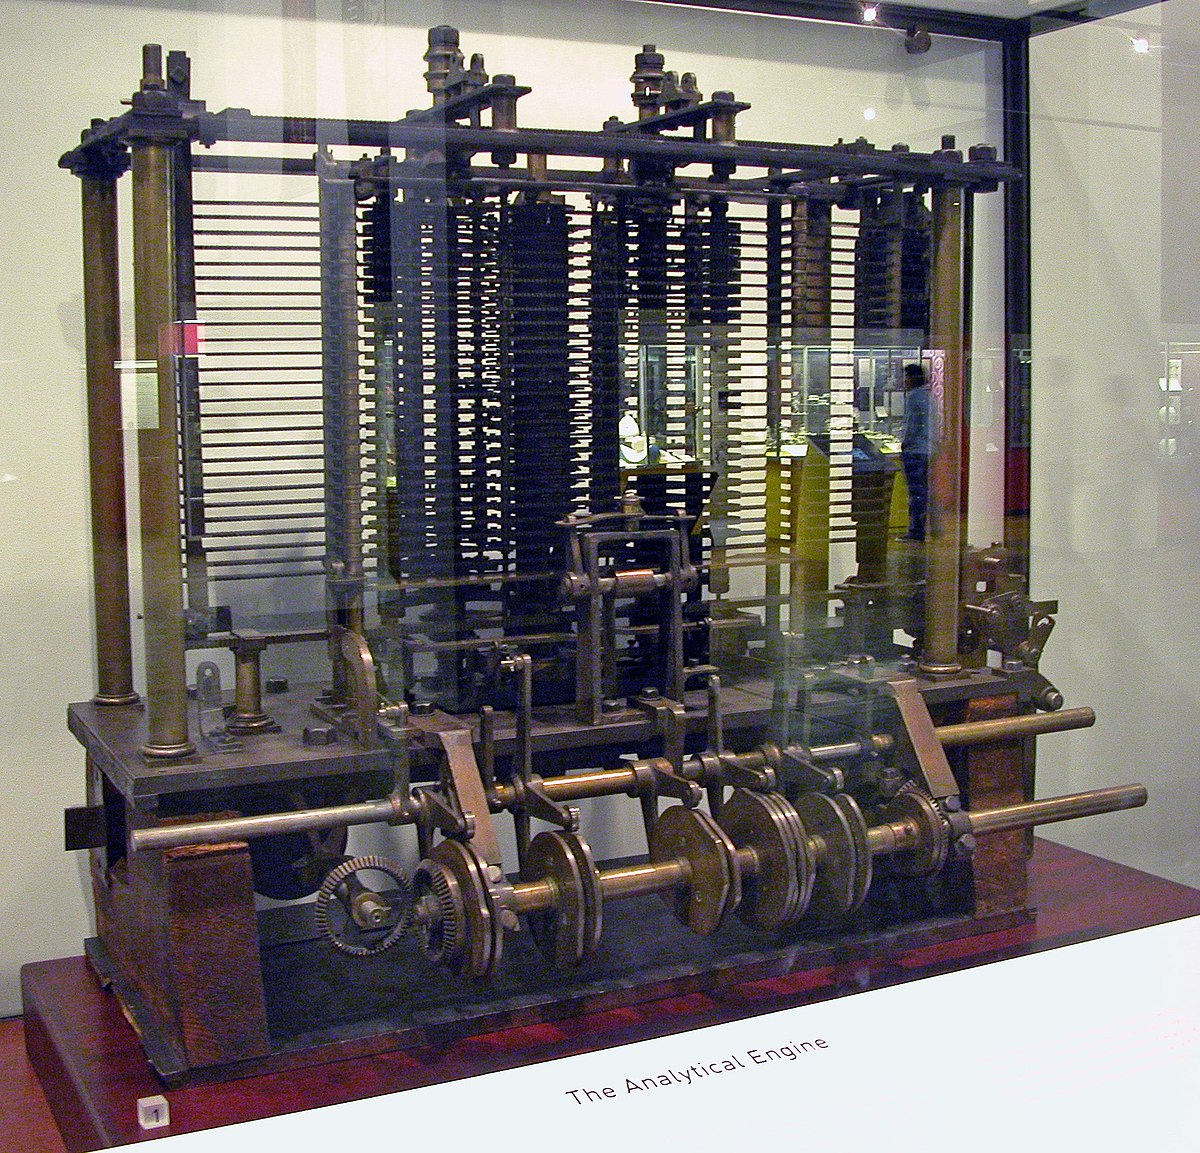
\includegraphics[width=0.7\linewidth]{Analitico.jpg}
\caption{Máquina Analítica}
\label{analitica}
\end{figure}


%%%%%%%%%%%%%%%%%%%%%%%%%%%%%%%%%%%%%%%%%%%% CAPITULO 4 - PRIMEIRA GERAÇÃO

\chapter{Primeira Geração de Computadores (1937-1956)}
\label{chap.PG}
\section{Características do \textit{hardware} e \textit{software}}
\paragraph{}
A primeira geração de computadores teve inicio na década de 30 do século \textit{XX}, sendo que esta geração apresentava poucas semelhanças aos computadores modernos, quer em aparência quer em performance.
Os primeiros computadores desta geração tinham um circuito constituido por  \hyperref[sec:valvulas]{\textbf{\textit{válvulas termiônicas}}}, e uma memória constituida por dispositivos de armazenamento denominados de \hyperref[sec:memoria]{\textbf{\textit{memória de tambor}}}.
\paragraph{}
Dado que o \textit{input} era realizado através de cartões perfurados e o \textit{output} era através de impressões, os operadores demoravam bastante tempo a configurar novos problemas.
Como os circuitos eram constituidos por \hyperref[sec:valvulas]{\textbf{\textit{válvulas termiônicas}}}, estes computadores sobreaqueciam frequentemente e tinham muitas vezes um tamanho considerável, com alguns dos maiores a ocupar salas inteiras e a pesar várias toneladas. Era muito dispendioso manter e operar um computador desta geração, pois gastavam muita energia e requeriam manutenção constante. \newline
A nível de software, dependiam de \hyperref[sec:codigo]{\textbf{\textit{código máquina}}} para realizar operações e só conseguiam resolver um problema de cada vez.


\subsection{Válvulas Termiônicas} 
\label{sec:valvulas}
\paragraph{}
Tendo um desenvolvimento desempenhado por vários cientistas ao longo dos anos, as\textbf{\textit{válvulas termiônicas}}~\ref{valvula} \cite{Valvulas} foram completadas em 1906 pelo físico estadunidense \textbf{\textit{Lee De Forest}}. Eram constituidas por dois ou mais electrodos dentro de um tubo de metal/vidro a vácuo, podendo transmitir sinais elétricos.
\paragraph{}
Desempenharam um grande papel na evolução dos computadores, pois foram a primeira forma de tecnologia activa a ser usada e permitiram construir as formações da industria eletrónica. 
Sendo uma das peças chave usadas nos primeiros computadores, serviam de amplificadores e comutadores no circuito.

\begin{figure}[H]
\centering
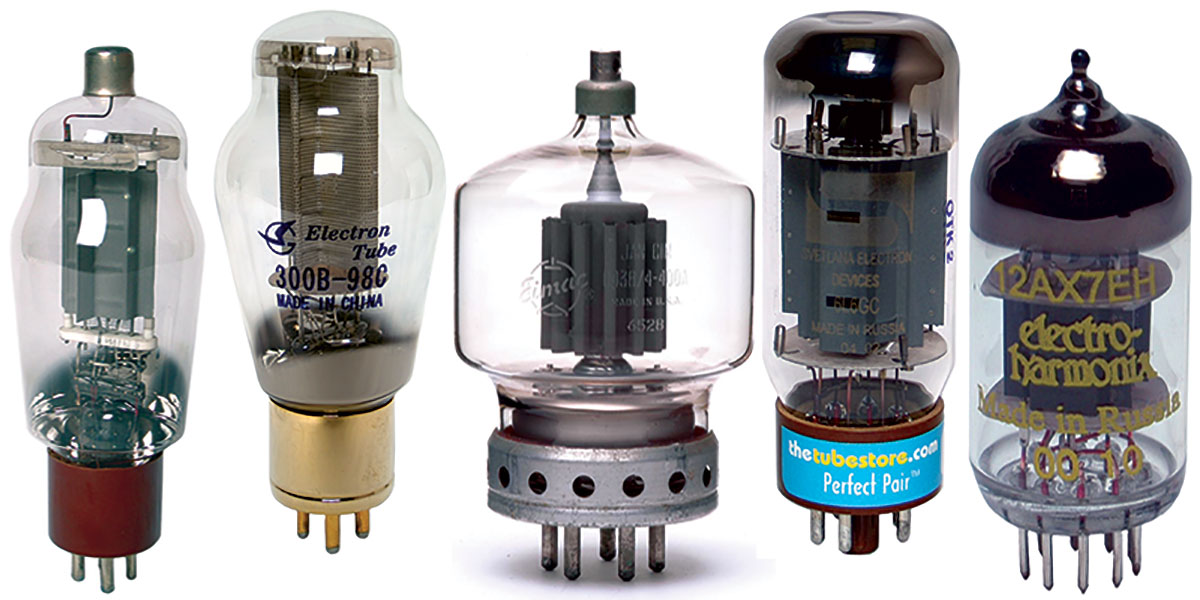
\includegraphics[width=0.5\linewidth]{VacuumTubes.jpg}
\caption{Válvulas Termiônicas}
\label{valvula}
\end{figure}

\subsection{Memória de Tambor} 
\label{sec:memoria}
\paragraph{}
As \textbf{\textit{memórias de tambor}}~\ref{tambor} \cite{Memoria} são dispositivos magnéticos de armazenamento de acesso direto. Capazes de recuperar informação a uma taxa de velocidade maior que acionadores de disco, foram usadas como armazenamento primário nos primeiros computadores.
Apesar disto, tinham várias desvantagens, como a impossibilidade de serem removidas após a instalação e tamanho de armazenamento reduzido.

\begin{figure}[H]
\centering
\includegraphics[width=0.3\linewidth]{MagneticDrum.jpg}
\caption{Memória de Tambor}
\label{tambor}
\end{figure}

\subsection{Código máquina} 
\label{sec:codigo}
\paragraph{}
A tecnologia de \textit{software} nesta época era bastante primitiva, o que obrigava a que os primeiros programas fossem escritos em \textbf{\textit{código máquina}} ou \textbf{\textit{linguagem máquina}} \cite{CodigoMaquina} .\newline
Esta linguagem é a de menor nível possível, a linguagem elementar dos computadores, e é constituida por uma sequência binária de 0s e 1s. Para realizar operações nestes computadores, os programadores escreviam diretamente os números que correspondiam ás instruções que tencionavam guardar na memória.

\section{Primeiro Computador Mecânico Programável em Binário}
\paragraph{}
Criado pelo alemão \textbf{\textit{Konrad Zuse}}, o \textbf{\textit{Z1}}~\ref{z1} \cite{Z1} foi o primeiro computador mecânico programável em binário. Construido no período de 1936-1938, foi o primeiro computador a usar lógica booleana e números com virgula flutuante, contudo era muito lento e muitas vezes inexato nos resultados.

\begin{figure}[H]
\centering
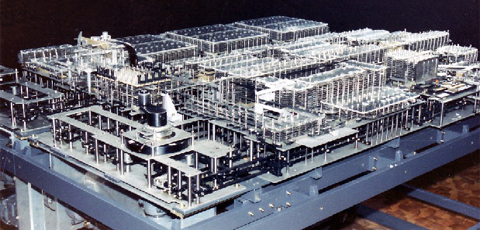
\includegraphics[width=0.7\linewidth]{Z1.jpg}
\caption{Computador Z1}
\label{z1}
\end{figure}

\section{Primeiro Computador Digital}
\paragraph{}
O \textbf{\textit{\acs{eniac}}}~\ref{eniac} \cite{ENIAC} foi o primeiro computador digital programável e totalmente funcional. Originalmente criado para ajudar os \acs{eua} a fazer cálculos relacionados com a balística na Segunda Guerra Mundial, a sua construção começou em 1943, porém só teria fim em 1946, um ano após o cessar fogo.
Com um peso de de 30 toneladas, sendo preciso uma sala inteira para o acomodar, este computador era capaz de realizar 5000 operações por segundo, resolvendo as quatro operações aritméticas e raizes quadradas, dando a resposta através de uma sequência de lâmpadas. Podia ser programado para resolver sequências de instruções complexas, incluindo \textit{loops}, \textit{branches} e sub-rotinas. 

\begin{figure}[H]
\centering
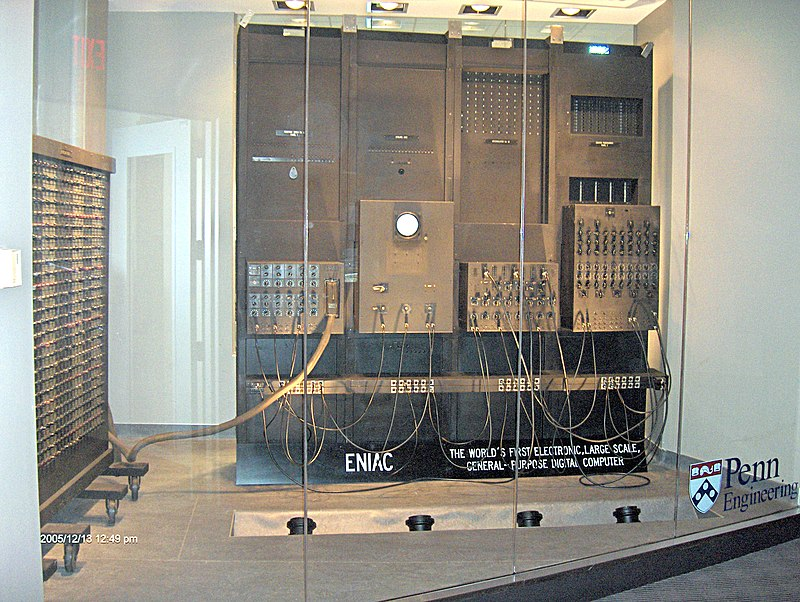
\includegraphics[width=0.7\linewidth]{ENIAC.jpg}
\caption{ENIAC}
\label{eniac}
\end{figure}

\section{Resumo da 1º Geração}

\begin{itemize}
\item Maior poder de computação alguma vez obtido
\item Uso de válvulas termiônicas 
\item Armazenamento primário através de memórias de tambor
\item Portabilidade muito reduzida devido ao tamanho e peso
\item Utilização e manutenção muito dispendiosa
\item Suporte exclusivo de linguagem máquina
\item Memória reduzida
\item \textit{Input} e \textit{output} muito lentos
\end{itemize}

%%%%%%%%%%%%%%%%%%%%%%%%%%%%%%%%%%%%%%%%%%%% CAPITULO 5 - SEGUNDA GERAÇÃO

\chapter{Segunda Geração de Computadores (1956-1965)}
\label{chap.SG}
\section{Características do \textit{hardware} e \textit{software} }
\paragraph{}
A segunda geração de computadores foi marcada por importantes desenvolvimentos a todos os níveis de \textit{design} do computador, desde a tecnologia usada nos circuitos básicos às linguagens de programação utilizadas.
Uma das mudanças mais signficativas foi a substituição das \hyperref[sec:valvulas]{\textbf{\textit{válvulas termiônicas}}} por dispositivos chamados \hyperref[sec:transistor]{\textbf{\textit{transístores}}}. Bastantes superiores á tecnologia usada até ao momento, os \hyperref[sec:transistor]{\textbf{\textit{transístores}}} permitiram construir computadores mais rápidos, duráveis e mais eficientes doque os seus antecessores. Contudo, ainda dependiam de cartões perfurados para fazer o \textit{input} e impressões para fazer o \textit{output}.
\paragraph{}
Esta foi a primeira geração a armazenar instruções na sua memória, que passou a ser constituida por \hyperref[sec:nucleo]{\textbf{\textit{memória de núcleos magnéticos}}}. Adicionalmente, os programadores deixaram de trabalhar em \hyperref[sec:codigo]{\textbf{\textit{código máquina}}}, adotando uma linguagem simbólica que permitia especificar instruções por palavras, a chamada linguagem do tipo \textit{Assembly}.

\newpage

\subsection{Transístor}
\label{sec:transistor}
Desenvolvidos por \textbf{\textit{John Bardeen}}, \textbf{\textit{Walter Brattain}} e \textbf{\textit{William Shockley}} em 1947, os \textbf{\textit{transístores}}~\ref{trans} \cite{Transistores} são dispositivos semicondutores, capazes de amplificar, controlar e gerar sinais elétricos. 
\paragraph{}
Usados diretamente nos computadores de segunda geração, e como iremos ver mais à frente, nas restantes gerações em forma de circuitos integrados, os \textbf{\textit{transístores}} funcionam como um \textit{switch} que age de acordo com a corrente. Se existe passagem de corrente elétrica, o circuito está ligado(\textit{on)}, caso contrário está desligado(\textit{off)}. Estes dois estados  correspondem aos números binários 0 e 1, que é a maneira como o computador comunica e lida com lógica \textit{booleana}.

\begin{figure}[H]
\centering
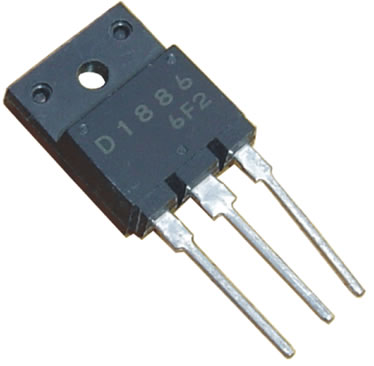
\includegraphics[width=0.2\linewidth]{transistor.jpg}
\caption{Transístor}
\label{trans}
\end{figure}

\subsection{Memória de Núcleos Magnéticos}
\label{sec:nucleo}
Os computadores da segunda geração foram os primeiros a usar esta memória, chamada de \textbf{\textit{memória de núcleos magnéticos}}~\ref{magn} \cite{memoriamagnetica}. Do tipo \acs{ram}, era constituida por um \textit{array} de núcleos de \textit{ferrite}, cada um capaz de armazenar 1 bit, e um conjunto de três fios que passavam por entre cada núcleo e que permitiam escrever e ler informação.
Demonstraram ser de grande uso na época mas, eventualmente, na década de 70, iriam deixar de ser utilizadas em favor das \acs{dram}.

\begin{figure}[H]
\centering
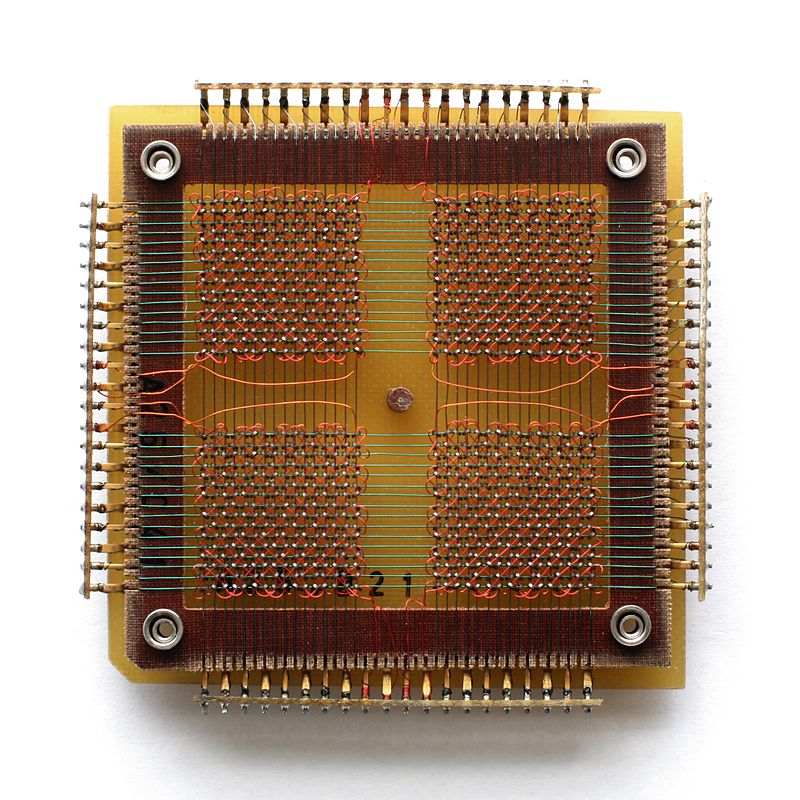
\includegraphics[width=0.2\linewidth]{memoriamagnetica.jpg}
\caption{Memória de núcleos magnéticos}
\label{magn}
\end{figure}


\subsection{Resumo da 2º Geração}
\begin{itemize}
   \item Substituição das válvulas termiônicas por transístores
   \item Armazenamento primário através de memória de núcleos magnéticos
   \item Suporte de linguagem máquina e linguagem do tipo \textit{Assembly}
   \item Redução de
   \begin{itemize}
     \item Peso
     \item Tamanho
     \item Consumo elétrico
   \end{itemize}
   \item Maior 
   \begin{itemize}
   \item Rapidez
   \item Capacidade de memória
   \end{itemize}
\end{itemize}


%%%%%%%%%%%%%%%%%%%%%%%%%%%%%%%%%%%%%%%%%%%%%%%%%%% CAPITULO 6 - TERCEIRA GERAÇÃO
\chapter{Terceira Geração dos Computadores (1965 - 1971)}
\label{chap.TG}
			
\paragraph{}
A  \textbf{\textit{terceira geração de computadores}}\cite{terceirageracao} teve em início em 1965 e teve como principal destaque a implementação de \textbf{\textit{circuitos integrados}}. \newline
A ideia dos circuitos integrados começou a ser desenhada por \textbf{\textit{Geoffrey W. A. Dummer}} na década de 50. \textbf{\textit{Dummer}}, para propagar e dar a conhecer a sua ideia, deu várias palestras e só em 1958, juntamente, com \textbf{\textit{Robert Noyce}}, \textbf{\textit{Jean Hoerni}}, \textbf{\textit{Jack Kilby}} e \textbf{\textit{Kurt Lehovec}} é que se iniciaram os desenvolvimentos dos \textbf{\textit{circuitos integrados}}.

\section{Circuitos Integrados}
\label{sec:circuitos}
\paragraph{}
Estes eram compostos por unidades de encapsulamento semicondutoras que agrupam \hyperref[sec:transistor]{\textbf{\textit{transístores}}}, resistores, diodos e outros componentes elétricos interligados entre si e que viriam a ser conhecidos como chips. Na altura havia duas variedades de \textbf{\textit{circuitos integrados}}, os \acs{ssi} (cerca de 10 transistores por chip) e os \acs{msi} (cerca de 100 transistores por chip).
\paragraph{}
O aparecimento dos \textbf{\textit{circuitos integrados}} e o desuso de \hyperref[sec:transistor]{\textbf{\textit{transístores}}} trouxe enúmeras vantagens ao mundo da computação. Esta troca possibilitou uma diminuição do tamanho dos computadores, do aquecimento e do consumo de energia. A próximidade dos circuitos possibilitou um aumentos da velocidade de processamentos dos computadores, origiando a mais operações por segundo. O processo de fabricação de \textbf{\textit{circuitos integrados}} era mais facilitado, ou seja, a sua produção em massa era muito maior e este avanço permitiu a que empresas, universidades e centros de pesquisa de médio "porte" pudessem ter este tipo de equipamento fazendo com que os computadores nao fossem exclusivos para uso militar e científico. O uso domiciliário ainda era um horizonte um pouco longuínquo porque os computadores, apesar do avanço significativo que tiveram, ainda eram robustos e muito dispendiosos a nivel energético.
\paragraph{}
Os primeiros computadores a terem \textbf{\textit{circuitos integrados}} a serem criados foram os modelos B3500 e o B3600 e foram ambos produzidos pela Burroughs Corporation e os computadores da linha \acs{ibm} System/360 que foram um sucesso de vendas, vendendo milhares de K350.\newline
Durante a década de 60, mais precisamente em 1968, foi criado, pelo Instituto de Pesquisas de Stanford, o primeiro rato. Este era constituido apenas por um botão e era feito em madeira. Nesta altura o armazenamento era feito por fita magnética, que é uma memória não volátil.

\section{Novas Linguagens de Programação}
\paragraph{}
Com esta vasta mudança de \textit{hardware} também vieram mudanças a nível de \textit{software}. Depois da criação de linguagens de baixo nível do tipo \textit{Assembly}, no início da década de 60 surgiram as primeiras linguagens de alto nível como \textbf{\textit{COBOL}}, \textbf{\textit{FORTRAN}} e \textbf{\textit{ALGOL}}. 

\section{Lei de Moore:}				
\paragraph{}
Em 1965, para acompanhar o progressivo crescimento dos \hyperref[sec:circuitos]{\textbf{\textit{circuitos integrados}}}, surgiu a \textbf{\textit{Lei de Moore}} \cite{leidemoore}. Esta lei estabelecia uma pseudo-regra para a evolução dos computadores que dizia que em cada 18 meses o número de \hyperref[sec:transistor]{\textbf{\textit{transistores}}} dos chips aumentava para metade mas mantendo o mesmo custo. Esta lei com o passar dos tempo foi se tornando cada vez mais real, pois sem ela, talvez não tivéssemos um crescimento tão acelarado do \textit{hardware} a preços cada vez mais acessíveis ao consumidor final.
Nos tempos que correm cada vez é mais provável que a \textbf{\textit{Lei de Moore}} acabe, pois os engenheiros estão a desenvolver sistemas que exigem menos recursos do processador e os custos associados a novas pesquisas de processadores estão cada vez mais altos. 

\section{Resumo da 3º Geração }
\begin{itemize}
	\item Implementação de circuitos integrados;
	\item Redução do tamanho;
	\item Menos calor gerado;
	\item Aumento de velocidade de processamento;
	\item Processo de fabrico mais facilitado;
	\item Criação de lingaguens de baixo nível;
	\item Implementação da Lei de Moore;
\end{itemize}

\section{Curiosidade:}
\paragraph{}
Na década de 60, como já sabemos, houve um abanão muito grande no mundo dos computadores e com isto os sistemas operativos também foram "vítimas" deste abanão. 
É nos anos 60 que surge a base do  \textbf{\textit{UNIX}}, que futuramente viria a ser o pai de praticamente todos os \acs{so}'s que existem hoje em dia. O \textbf{\textit{UNIX}}foi criado por \textbf{\textit{Kenneth Thompson}}, \textbf{\textit{Dennis Ritchie}}, entre outros, e foi escrito em \textbf{\textit{C}}, algo que é apontado para a justificação do seu grande sucesso.

\newpage

\chapter{Quarta Geração dos Computadores (1971 - 1981)}
\label{chap.QG}
\paragraph{}
O que marcou o início da \textbf{\textit{quarta geração de computadores}}~\cite{quartageracao} foi o lançamento do primeiro \textbf{\textit{microprocessador}} comercial.\newline
 Esta pequena peça foi desenvolvida pela \textbf{\textit{Intel}} e ficou denominada por \textbf{\textit{Intel 4004}} que era muito mais potente que os circuitos \acs{ssi} e \acs{msi} criados na terceira geração. O \textbf{Intel 4004} veio por consequência de um desenvolvimento do estudo dos \hyperref[sec:circuitos]{\textbf{\textit{circuitos integrados}}}, e foi criado por \textbf{\textit{Federico Faggin}}, \textbf{\textit{Ted Hoff}} e \textbf{\textit{Stanley Mazor}}.
\paragraph{}
A continuidade do projeto de miniaturização deu origem aos circuitos integrados \acs{lsi}(mil transistores por chip) e os \acs{vlsi} e esses novos circuitos passaram a ser chamados de \textbf{\textit{microprocessadores}}. Como cada vez mais as componentes de um computador iam diminuido de tamanho e este, por consequência, também ia diminuindo cada vez mais, chegando a ser chamado de microcomputador.	A velocidade dos processadores e a capacidade de memória também aumentaram. Porém, um dos principais avanços desta quadra foi o surgiemento da teleinformática, e tinha como características a transmissão de dados por via de uma rede.

\begin{figure}[H]
\centering
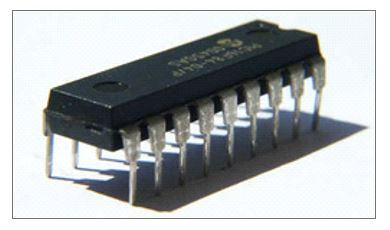
\includegraphics[width=0.6\linewidth]{fig2.png}
\caption{Microprocessador}
\end{figure}

\begin{figure}[H]
\centering
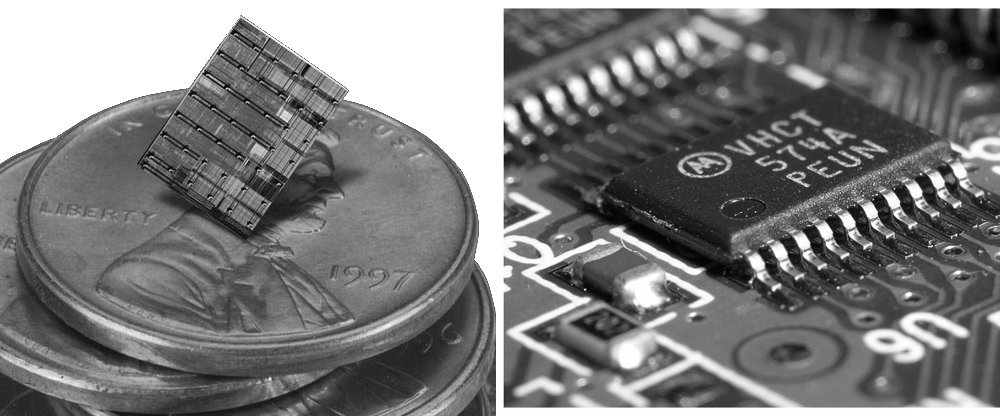
\includegraphics[width=0.6\linewidth]{fig1.png}
\caption{Microprocessador em comparação com uma moeda}
\end{figure}


\section{A Internet}
\paragraph{}
A \textbf{\textit{internet}}\cite{internet}, que hoje conhecemos, é algo que nos é "essencial". Usamos todos dias quer seja para ler notícias , para ver videos, para trabalhar ou para navegarmos nas redes sociais. Mas tudo o que temos hoje foi fruto de largos anos de trabalho por parte de engenheiros que desenvolverem a internet até aquilo que nos deparamos agora.
\paragraph{}
Tudo começou em 1969 onde foi criado um projeto denominado de \textbf{\textit{ARPANET}}~\cite{ARPANET}. Este projeto teve uma duração de 3 anos e foi o estudo que deu início à \textbf{\textit{internet}}. A \textbf{\textit{ARPANET}} foi a primeira rede operacional de computadores à base de comutação de pacotes sendo usada só para fins militares. Esta pequena rede tinha apenas 4 computadores localizados na Universidade da Califórnia, em Santa Bárbara no Stanford Research Institute e na Universidade do Utah. A sua primeira operação foi um Log In realizado entre a Universidade da Califórnia e o Stanford Research Institute, infelizmente, esta ligação não foi bem sucessida. Só em 1972 é que o \textbf{ARPANET} foi realmente apresentado por \textbf{\textit{Robert Khan}} na Conferência Internacional de Computadores. 
\paragraph{}
Por volta dos anos 70 surgiu a \textbf{\textit{Ethernet}}, um conceito de rede local. De seguida foi criado o protocolo TCP/IP que acabou por se tornar o protocolo definitivo para o uso da \textbf{\textit{ARPANET}}e ainda utilizado nos dias de hoje. 
No final da década de 70, aproximadamente, 200 computadores já estavam ligados à \textbf{\textit{ARPANET}} devido ao uso por parte da comunicação militar durante a Guerra Fria. No final da guerra a \textbf{\textit{ARPANET}} foi passada às universidades porque já não era do interesse militar usar o serviço. Com a expansão da rede por parte dos pesquisadores e das universidades, no final dos anos 70 e inícios dos anos 80 a \textbf{\textit{ARPANET}} já contava com mais de 100 mil dispositivos ligados entre si, criando, deste modo, uma gigante rede mundial intitulada como conhecemos hoje de, \textbf{\textit{internet}}
\paragraph{}
O destaque da década de 90 vai para a criação da \textbf{\textit{World Wide Web}}, projeto desenvolvido no \acs{cern}, pelo cientista \textbf{\textit{Timothy John Berners Lee}}.
\textbf{\textit{Tim Berners}} e os seus colegas foram os pioneiros na criação das versões iniciais de \textbf{\textit{HTML}} e do \textbf{\textit{HTTP}}. No ano de 1993, houve uma grande viragem no mundo da web com a criação e introdução do primeiro browser, \textbf{\textit{Mosaic}}.\\As evoluções da internet não ficaram por aqui, foram criados \textit{updates} ao longo dos anos para que os clientes e usuários da \textbf{\textit{internet}} possam ter uma melhor utilização daquilo que é das coisas mais imporantes no nosso quotidiano. 

\section{Continuação da Inovação}
\paragraph{}
A a partir de 1971, vários computadores foram desenvolvidos por várias marcas entre elas a \acs{ibm}, a \textbf{\textit{Xerox}} e a \textbf{\textit{Apple}}.
Em 1971, a \acs{ibm}, criava o primeiro computador com a memória central ligeiramente constituída por tecnologia monolítica. De seguida, em 1973, foi criado o Xerox Alto, um microcomputador que utilizava uma interface gráfica de usuário e o primero \textit{desktop} pessoal. \newline
Em 1976, \textbf{\textit{Stephen Wozniak}}, ex-funcionário da \acs{hp}, e \textbf{\textit{Steve Jobs}}~\ref{Steve}, da \textbf{\textit{Atari}}, uniram-se e criaram a tão famosa empresa, \textbf{\textit{Apple}}. Em conjunto, produziram o primeiro microcomputador de grande sucesso, o \textbf{\textit{Apple I}}~\ref{Apple}, que foi considerado o primeiro computador pessoal.
\paragraph{}
Com o avançar da tecnologia muitas pessoas começaram a ter acesso a computadores com o baixar do seu preço isto implicou uma mudança de software porque este precisava de ser menos complexo e foi aí que começaram a surgir os Sistemas Operativos.\newline
Os primeiros sistemas operativos eram sistemas que apenas permitiam ao usuário realizar uma única tarefa de cada vez, de seguida surguiram os sistemas operativos multitarefas, o \textbf{\textit{Microsoft Windows}} e o \textbf{\textit{MacOS}} são exemplos desses sistemas. O \textbf{\textit{MS-DOS}} da \textbf{\textit{Microsoft}} e o \textbf{\textit{UNIX}} foram sistemas operacionais que tiveram muito em voga nos computadores pessoais. De seguida, surgiu o \textbf{\textit{Windows}} que era mais uma \textit{shell} do que um sistemas operativo, com isto, criou-se o \textbf{\textit{Windows 95}} que veio substituir o \textbf{\textit{MS-DOS}}. \newline
No ano de 1972, é criada a primeira versão da linguagem de programação \textbf{\textit{C}}.

\begin{figure}[h]
	\centering
	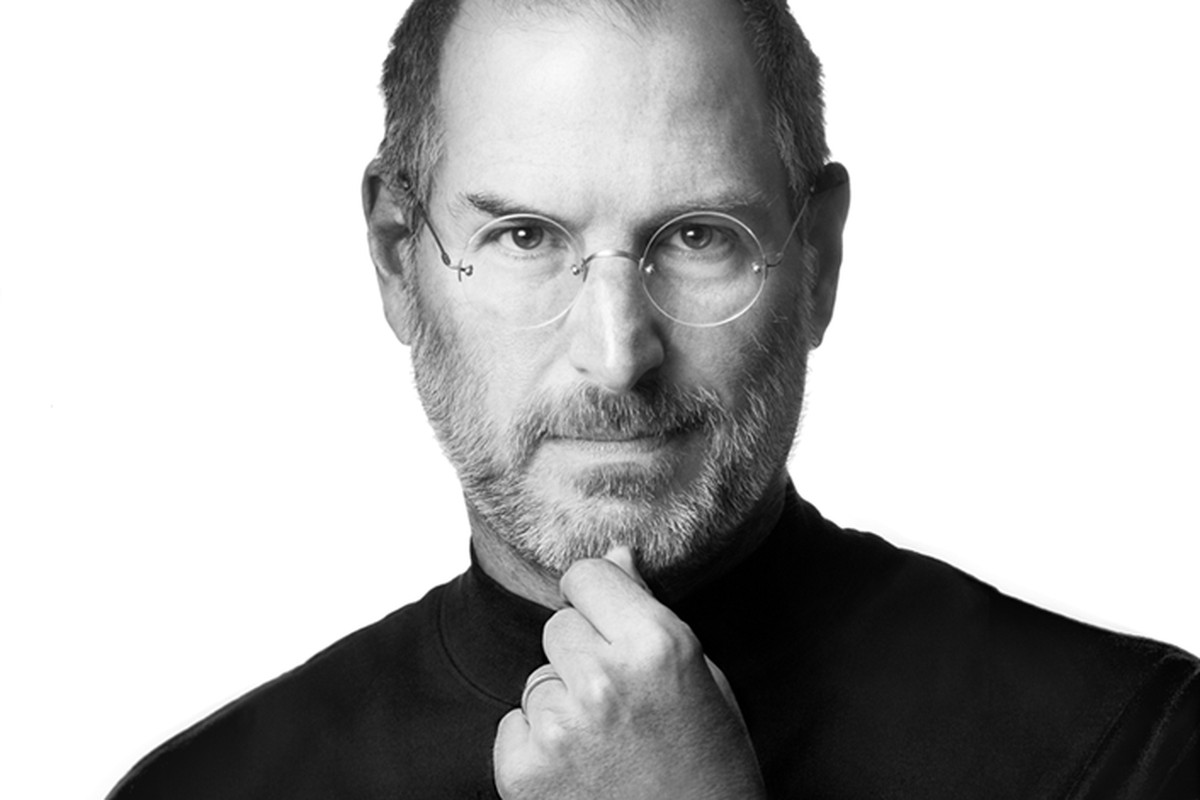
\includegraphics[scale=0.15]{fig5.png}
	\caption{Steve Jobs}
	\label{Steve}

\end{figure}

\begin{figure}[h]

	\centering

	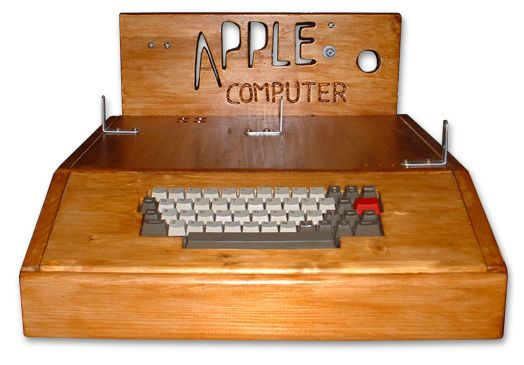
\includegraphics[scale=0.15]{fig4.png}
	\caption{Apple I}
	\label{Apple}

\end{figure}

\section{Resumo da 4º Geração}

\begin{itemize}
	\item Introdução dos microprocessadores;
	\item Criação e aperfeioamento da Internet;
	\item Desenvolvimento dos primeiros computadores pessoais;
	\item Desenvolviemnto do software;
	\item Criação de novos Sistemas Operativos (MS-DOS, Windows, UNIX, MacOS);
	\item Criação de novas linguagens de programação;
\end{itemize}	

%%%%%%%%%%%%%%%%%%%%%%%%%%%%%%%%%%%%%%%%%%%%%%% CAPITULO 5 - QUINTA GERAÇÃO
\chapter{Quinta Geração dos Computadores (1981 - Actualidade)}
\label{chap:IA}
\paragraph{}
A quinta geração\cite{quintageracao} da história dos computadores deve o seu nome a um grande projeto, por parte do governo e da indústria do Japão durante a década de 80. O principal objetivo desta investigação era a criação de um computador que marcasse uma geração. A quinta geração prometia convencionar todo um novo sistema da tecnologia querendo deixar, deste modo, as máquinas passadas obsoletas. Esta, ambiação, tão grande,  do Japão de avançar na tecnologia em relação aos outros países era porque até lá o Japão tinha estado na retaguarda de países como a Inglaterra ou os Estados Unidos da América.
\paragraph{}
Esta ambição levou a que o ministro da indústria e dos negócios estrangeiros fizesse um pedido ao Centro Japonês para o Desenvolvimento do Processamento da Informação para fazer um estudo dos caminhos a seguir para tomar a dianteira do mercado informático.
Entretanto, no outro lado do mundo eram criados dois computadores importantíssims na nossa história mundial. Em 1981, era criado o \textbf{\textit{\acs{ibm}}} \textbf{\textit{Personal Computer 5150}}~\ref{5150}. Dois anos mais tarde a \textbf{\textit{Apple}}, lançava um computador revolucionário, o \textbf{\textit{Apple Lisa}}~\ref{lisa} . Este computador viria a ser um fracasso pelo seu preço, extremamente, alto e pela sua configuração ser considerada "extravagante" para a época. 
			
\begin{figure*}[h]

	\centering 
	\begin{minipage}[b]{.48\textwidth}
	
		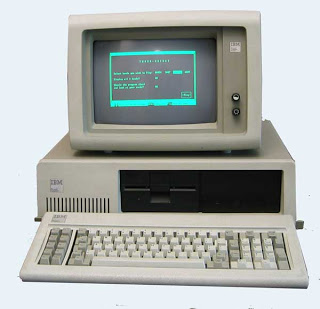
\includegraphics[width = 1\linewidth]{fig6.png}		
		\caption{IBM 5150}
		\label{5150}
		
	\end{minipage}	
%	\qquad
	\begin{minipage}[b]{.48\textwidth}
	
		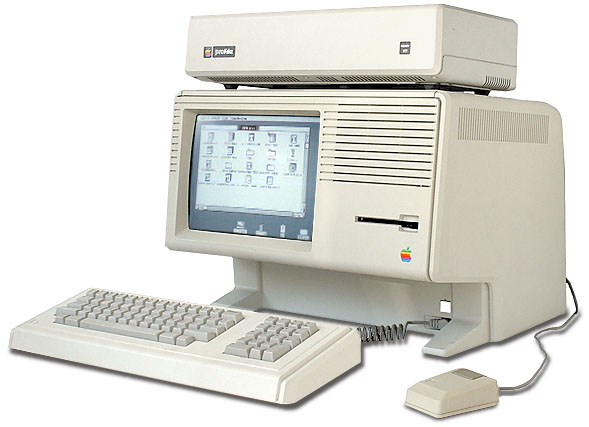
\includegraphics[width = 1\linewidth]{fig7.png}
		\caption{Apple Lisa}
		\label{lisa}
		
	\end{minipage}	
			
\end{figure*}

Como todas a gerações as gerações tiveram problemas e obstáculos a quinta nao foi exeção. O primeiro problema assentava na linguagem de programação \textbf{\textit{prolog}} e residia no facto de esta não oferecer suporte para concorrênicas. Isto obrigou à criação de novas linguagens mas todas elas tinham as suas próprias limitações. Um grande outro problema foi as performances das \acs{gpu} e o valor da computação paralela, caiu de forma rápida para o ponto que ainda hoje em dia é utilizada, mas o que é isto da computação paralela? 
\paragraph{} 
A \textbf{\textit{computação paralela}} \cite{computacaoparalela} é uma forma de computação onde diversos cálculos sao realizados ao mesmo tempo, operando do princípio em que os grandes problemas podem ser dividios, de forma geral, em problemas mais pequenos. Neste momento, exitem vários tipo de computação paralela: em bit, instrução, de dado ou de tarefa.
Foi na quinta geração que, foi introduzida a \textbf{\textit{\acs{gui}}}. Esta foi criada pela \textbf{\textit{Xerox}} mas só foi comercializada pela \textbf{\textit{Apple}} e só aí é que se tornou um produto.	
			
\section{Inteligência Artificial:}		
\paragraph{}	
Um dos marcos mais importantes da quinta geração foi a \textbf{\textit{Inteligência Artificial}} \cite{artificial}. Esta ramificação do ramo da ciência computacional propõe conceber dispositivos que simulem a capacidade humana de racicionar, tentando atuar, no final, como um ser humanao inteligente. A principal característica de um sistema com inteligência artificial é que o sistema reconhece o seu ambiente e toma atitudes para que maximize as suas chances de sucesso. Podemos pensar em algumas componentes básicas destes sistemas, como a capacidade de raciocínio (usar regras lógicas para chegar a uma conclusão), aprendizagem (aprender com os erros e acertá-los se forma a agir mais corretamente no futuro), reconhecer padrões ( padrões visuais, sensoriais e de comportamento) e inferência ( capacidade de aplicar o raciocínio no dia-a-dia).
\paragraph{}
O desenvolviento desta área deu-se logo a seguir à Segunda Guerra Mundial ter acabado com um artigo chamado \textit{"Computing Machinery and Intelligence"} do famoso matemático \textbf{\textit{Alan Turing}} mas só agora é que  ganhou meios para, realmente, se desenvolver. Isto deve-se ao surgimento do computador moderno, algo que permitiu estudar de forma mais aprofundada este tema, que ainda hoje continua em aberto e a suscitar muita discussão.
\paragraph{}

Podemos dividor a \textbf{\textit{Inteligência Artificial}}l em três grandes aplicações:
\begin{itemize}
			\item Os processos de linguagem natural, que facilita a comunicação do computador com o utilizador;
			\item A robótica e tudo associado à visão e manipulação de objetos;
			\item Os sistemas especialistas, baseados no armazenamento do conhecimento adquirido;
\end{itemize}	


\section{Resumo da 5º Geração :}
\begin{itemize}
		\item  Impulsão do Japão no negócio computacional;
		\item Criação dos primeiros computadores pessoais;
		\item Desenvolvimento de novas linguagens de programação 
		\item Inteligência Artifical;
\end{itemize}

\newpage

\chapter{Conclusão:}
\label{chap:conclusao}
\paragraph{}	
Vivemos num mundo em constante alteração, quer seja na informática, quer seja na ciência, quer seja na medicina, etc. Toda a história aqui traçada remonta a grandes feitos e a grandes homens que mudaram o rumo da nossa humanidade para sempre. Hoje em dia vivemos arrados a esses feitos porque o computador, cada vez mais, faz parte do ser humano e facilita-nos em tudo. Com este trabalho ficamos muito mais elucidados daquilo que temos nas mãos e do desenvolvimento que teve ao longo dos anos. 

\newpage
\section{Contribuição dos autores}
\paragraph{}
O aluno Pedro Rocha ficou encarregue da terceira geração, quarta geração, quinta geração e conclusão.
\paragraph{}
O aluno Luis Couto ficou encarregue da capa, titulo, resumo, introdução, metodologia, mecanismos de computação, primeira geração e segunda geração.
\paragraph{}
Tendo isto em conta, a contribuição de PR foi 50\% e de LC foi 50\%
 

%%%%%%%%%%%%%%%ACABA

\printbibliography

\end{document}


